%\documentclass[a4paper]{article}
\documentclass[landscape,twocolumn,a4paper]{article}
\usepackage[a4paper,vmargin={20mm,20mm},hmargin={20mm,10mm}]{geometry}

\author{Simon Wehrli}
\date{11.5.2013}
\title{Set similarity with k-permutation Minwise Hashing - NOTES}

\usepackage[parfill]{parskip}
\usepackage{tikz} % for drawing advanced matrices
\usepackage{amsmath}
\usepackage{amsthm}
\usepackage{algorithm}
\usepackage{algorithmicx}
\usepackage{algpseudocode}
\usepackage{natbib}
\usepackage{tabulary}
\usepackage{caption}
\usepackage{framed}
\usepackage[english]{varioref} %automatische Anpassung von Referenzen
\labelformat{equation}{(#1)} %make references to equations like (1)
\usepackage{float} % bewirkt, dass Option [H] für float-Umgebungen von Latex umgesetzt wird

\usetikzlibrary{matrix,decorations.pathreplacing,backgrounds,positioning}

\DeclareMathOperator{\Var}{Var}
\DeclareMathOperator{\E}{E}

\renewcommand{\algorithmicrequire}{\textbf{Input:}}
\renewcommand{\algorithmicensure}{\textbf{Output:}}

\newtheorem{mydef}{Definition}
\newtheorem{mylemma}{Lemma}
\newtheorem{mytheorem}{Theorem}

\newcommand*{\bfrac}[2]{\genfrac{\lbrace}{\rbrace}{0pt}{}{#1}{#2}}

\begin{document} 
\maketitle

\section{Introduction}
Many today's applications are faced with very large datasets. A common task is to find \emph{similarity} between two or several such sets.

This notes are intended as a help for the talk and explains only the core concepts of \citep{LiK11} and \citep{LiOwZhang12}.

\subsection{Similarity}
We denote by $\Omega$ the set of all possible items of the sets $S_n \subseteq \Omega$, $n = 1 \text{ to } N$. $\left| \Omega \right| = D$ is always large (e.g. $D=2^{64}$). Often we consider only two sets $S_1 = X$, $S_2 = Y$. Let $a=|X \cap Y|,$ $b=|X|-a$ and $c=|Y|-a$. Figure \vref{fig:sets} summarizes these definitions graphically.

\begin{figure}[H]
\centering
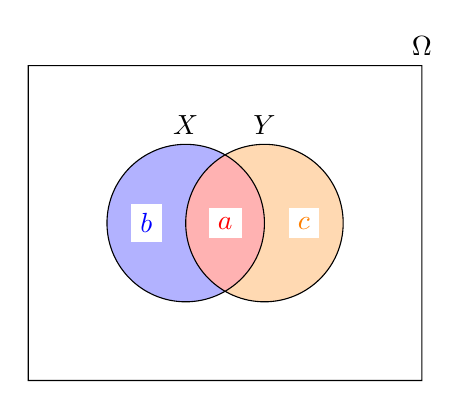
\begin{tikzpicture}
% left hand
\scope
\clip (-2,-2) rectangle (2,2)
      (1,0) circle (1);
\fill[fill=blue!30] (0,0) circle (1);
\endscope
% right hand
\scope
\clip (-2,-2) rectangle (2,2)
      (0,0) circle (1);
\fill[fill=orange!30] (1,0) circle (1);
\endscope
% middle
\scope
\clip (-2,-2) rectangle (2,2)
      (0,0) circle (1)
      (1,0) circle (1);
\fill[fill=red!30] (1,0) circle (1);
\endscope

% outline
\draw (0,0) circle (1) (0,1)  node [text=black,above] {$X$}
      (1,0) circle (1) (1,1)  node [text=black,above] {$Y$}
      (-2,-2) rectangle (3,2) node [text=black,above] {$\Omega$};
\node[draw=none,text=blue,fill=white] at (-0.5,0) {$b$};
\node[draw=none,text=red,fill=white] at (0.5,0) {$a$};
\node[draw=none,text=orange,fill=white] at (1.5,0) {$c$};
\end{tikzpicture}
\caption{Two example sets in $\Omega$ and the notation $a,b,c$ for the sizes of important subsets.}
\label{fig:sets}
\end{figure}

\begin{framed}
\begin{mydef}\label{def:jaccard}
The normalized similarity between two sets $X$ and $Y$, known as \emph{resemblance} or \emph{Jaccard similarity}, denoted by R, is
\begin{equation}
R=\frac{\left| X \cap Y \right|}{\left| X \cup Y \right|} = \frac{a}{\left| X \right| + \left| Y \right| -a}=\frac{a}{a+b+c}
\end{equation}
\end{mydef}
\end{framed}

\paragraph{Other Notations}
 
Later we often look at some important event of a problem where we use $\Pr[\cdot]$ as a shorthand for the \emph{Probability} of that event. To get an estimator for $R$ out of a probabilistic argument, we always use some Bernoulli experiment. This is a process, where we repeatedly flip a possibly biased coin, but the bias does not change. We can see it as a sequence of binary random variables, because only two outcomes are possible, $0$ or $1$. An event is described by an equation. We use the notation $1\left\lbrace \text{\textit{equation}} \right\rbrace$ which is one if and only if the \textit{equation} in curly braces is true:
\begin{equation*}
1\left\lbrace \text{\textit{equation}} \right\rbrace =\begin{cases}
    1 & \text{if \textit{equation} evaluates to \textit{true}} \\
    0 & \text{otherwise}
\end{cases}
\end{equation*}

\pagebreak

\section{Original Minwise Hashing}

Suppose a random permutation $\pi$ is performed on $\Omega$\footnote{We assume there is a perfect hash function applied to the elements of the original domain which always gives us $\Omega = \{0,1,\ldots,D-1\}$. Note that in the paper \citep{LiK11}, the hash function is applied after the permutation and the minimum-function, but it is simpler to understand this way.},
\[
\pi:\Omega \longrightarrow \Omega, \qquad \text{where } \Omega = \{0,1,\ldots,D-1\}.
\]

To simplify notation, we overload the definition of $\pi$ to work also for subsets of $\Omega$. Thus with $\pi(S_n)$ we denote the application of the permutation $\pi$ to every element of the set $S_n$. More precisely,
\begin{equation*}
\begin{split}
\pi &: 2^\Omega \longrightarrow 2^\Omega, \\
\pi &: S_n \longmapsto \pi \left( S_n \right) = \left\lbrace \pi \left( i \right) \middle\vert i \in S_n \right\rbrace. 
\end{split}
\end{equation*}

We define
\[
h_{S_n,\pi}=min(\pi(S_n))
\]
to be the smallest element of set $S_n$ permuted with $\pi_j$. Note that the smallest element changes under the permutations because $\pi$ is a permutation on $\Omega$ and $S_n$ is only a subset of $\Omega$ in general.

An elementary probability argument shows that for two sets $X,Y \subseteq \Omega$
\begin{equation}\label{eq:minwiseOri}
\Pr[h_{X,\pi}=h_{Y,\pi}]=\Pr [\min(\pi(X))=\min(\pi(Y))]=\frac{\left| X \cap Y \right|}{\left| X \cup Y \right|}=R.
\end{equation}

We can now build an unbiased estimator $\hat{R}_M$ of $R$ with $k$ minwise independent permutations, $\pi_1,\pi_2,\ldots,\pi_k$:
\begin{equation}
\hat{R}_M=\frac{1}{k}\sum_{j=1}^k 1 \left\lbrace h_{X,\pi_j}=h_{Y,\pi_j} \right\rbrace,
\end{equation}
\begin{equation}\label{eq:minWiseVariance}
Var(\hat{R}_M)=\frac{1}{k}R(1-R).
\end{equation}




\subsection{The Algorithm}

Based on the theoretical results, Algorithm \vref{alg:orgMinwiseHashing} presents the procedure of ($k$-permutation) \textsc{Minwise Hashing}.

\begin{algorithm}[H]
\caption{Original \textsc{Minwise Hashing} algorithm, applied to estimating pairwise resemblances in a collection of $N$ sets.}
\label{alg:orgMinwiseHashing}
\begin{algorithmic}
\Require Sets $S_n \subseteq \Omega = \{0,1,\ldots,D-1\}, n = 1 \text{ to } N$. \Comment $D = \left| \Omega \right|$
\Ensure Estimated resemblance $\hat{R}_M$
\State // Pre-processing
\State Generate $k$ random permutations $\pi_j: \Omega\longrightarrow\Omega, j=1\text{ to }k$
\ForAll{$n = 1 \text{ to } N, j = 1 \text{ to } k$}
	\State Store $\min(\pi_j(S_n))$, denoted by $h_{S_n,\pi_j}$.
\EndFor
\State
\State // Estimation (Use two sets $X,Y$ as an example)
\State Estimate the resemblance by $\hat{R}_M=\frac{1}{k}\sum_{j=1}^k 1 \left\lbrace h_{X,\pi_j}=h_{Y,\pi_j} \right\rbrace$
\end{algorithmic}
\end{algorithm}







\section{One Permutation Hashing}

This algorithm is directly motivated by the optimization potential of the standard \textsc{Minwise Hashing} method: intuitively, it ought to be ``wasteful'' in that all elements in a set are permuted, scanned but only the minimum will be used. As the name already suggests, we reduce the preprocessing step to only one permutation.

We will setup a running example with $X,Y,Z \subseteq \Omega = \left\lbrace 0,1,\cdots,15\right\rbrace$. Let be $\pi$ some random permutation on $\Omega$ and the already permuted sets be
\[
\pi(X)=\left\lbrace 2,4,7,13\right\rbrace, \quad \pi(Y)=\left\lbrace 0,3,6,13\right\rbrace,\quad \pi(Z)= \left\lbrace 0,1,10,12\right\rbrace.
\]
Now again we build up a data matrix where the rows are equal to the vector representations of the permuted sets:

\begin{equation}
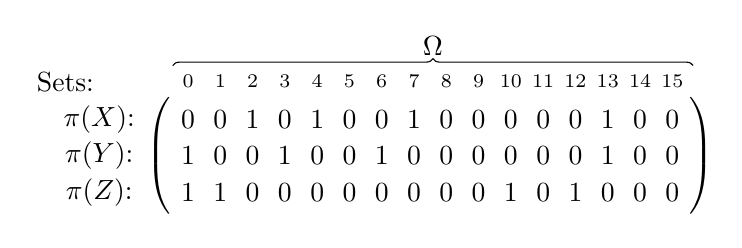
\begin{tikzpicture}[baseline = (M.center),% center with respect to the matrix center
        every left delimiter/.style={xshift=1ex},%tighter delimiter spacing
        every right delimiter/.style={xshift=-1ex}]
\matrix (M) [matrix of math nodes,left delimiter={(},right delimiter={)} 
        ]{ 
0&0&1&0&1&0&0&1&0&0&0&0&0&1&0&0\\
1&0&0&1&0&0&1&0&0&0&0&0&0&1&0&0\\
1&1&0&0&0&0&0&0&0&0&1&0&1&0&0&0\\
};
\node[anchor=south east] (cornernode) at (M-1-1.north west) {Sets: \qquad \qquad}; %Position this more precisely if desired
\foreach[count=\xi] \x in {0,1,2,3,4,5,6,7,8,9,10,11,12,13,14,15}{ %\xi is the counter \x is the value
\node[font=\scriptsize] (M-0-\xi) at (cornernode -| M-1-\xi) {\x}; % Gets the top row 
}

\foreach[count=\xi] \x in {$\pi(X)$:,$\pi(Y)$:,$\pi(Z)$:}{ %\xi is the counter \x is the value
\node (M-\xi-0) at (cornernode |- M-\xi-1) {\x}; %Gets the left most column
}

\draw[decoration=brace,decorate] (M-0-1.north west) -- (M-0-16.north east)%
 node[midway,above] {$\Omega$};

\end{tikzpicture}
\end{equation}

The idea is to divide the columns evenly into $t$ (here $t=4$) bins (parts), take the minimum in each bin. Because later we only compare minima within one bin, we can re-index the elements to use the smallest possible representation:

\begin{equation} \label{matrix:complete}
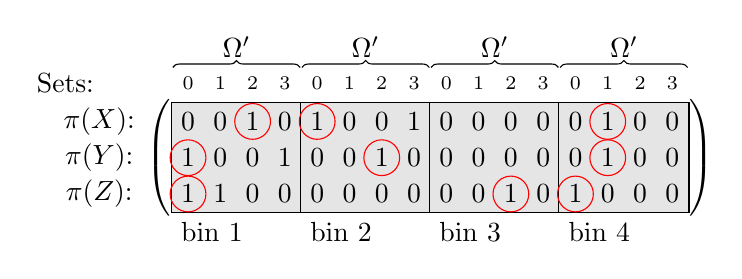
\begin{tikzpicture}[baseline = (M.center),% center with respect to the matrix center
        every left delimiter/.style={xshift=1ex},%tighter delimiter spacing
        every right delimiter/.style={xshift=-1ex}]
\matrix (M) [matrix of math nodes,left delimiter={(},right delimiter={)} 
        ]{ 
0&0&1&0&1&0&0&1&0&0&0&0&0&1&0&0\\
1&0&0&1&0&0&1&0&0&0&0&0&0&1&0&0\\
1&1&0&0&0&0&0&0&0&0&1&0&1&0&0&0\\
};
\node[anchor=south east] (cornernode) at (M-1-1.north west) {Sets: \qquad \qquad}; %Position this more precisely if desired
\foreach[count=\xi] \x in {0,1,2,3,0,1,2,3,0,1,2,3,0,1,2,3}{ %\xi is the counter \x is the value
\node[font=\scriptsize] (M-0-\xi) at (cornernode -| M-1-\xi) {\x}; % Gets the top row 
}
\foreach[count=\xi] \x in {$\pi(X)$:,$\pi(Y)$:,$\pi(Z)$:}{ %\xi is the counter \x is the value
\node (M-\xi-0) at (cornernode |- M-\xi-1) {\x}; %Gets the left most column
}
\node[below left = 0.1pt of M-3-3.south] {bin $1$};
\node[below left = 0.1pt of M-3-7.south] {bin $2$};
\node[below left = 0.1pt of M-3-11.south] {bin $3$};
\node[below left = 0.1pt of M-3-15.south] {bin $4$};

\draw[decoration=brace,decorate] (M-0-1.north west) -- (M-0-4.north east)%
 node[midway,above] {$\Omega'$};
\draw[decoration=brace,decorate] (M-0-5.north west) -- (M-0-8.north east)%
 node[midway,above] {$\Omega'$};
\draw[decoration=brace,decorate] (M-0-9.north west) -- (M-0-12.north east)%
 node[midway,above] {$\Omega'$};
\draw[decoration=brace,decorate] (M-0-13.north west) -- (M-0-16.north east)%
 node[midway,above] {$\Omega'$};

\begin{scope}[on background layer]
\draw [fill=black!10] (M-1-1.north west) rectangle (M-3-4.south east);
\draw [fill=black!10] (M-1-5.north west) rectangle (M-3-8.south east);
\draw [fill=black!10] (M-1-9.north west) rectangle (M-3-12.south east);
\draw [fill=black!10] (M-1-13.north west) rectangle (M-3-16.south east);
\draw [draw=red] (M-1-3.center) circle (1.5ex);
\draw [draw=red] (M-2-1.center) circle (1.5ex);
\draw [draw=red] (M-3-1.center) circle (1.5ex);
\draw [draw=red] (M-1-5.center) circle (1.5ex);
\draw [draw=red] (M-2-7.center) circle (1.5ex);
\draw [draw=red] (M-3-11.center) circle (1.5ex);
\draw [draw=red] (M-1-14.center) circle (1.5ex);
\draw [draw=red] (M-2-14.center) circle (1.5ex);
\draw [draw=red] (M-3-13.center) circle (1.5ex);
\end{scope}
\end{tikzpicture}
\end{equation}

We get the minima-vectors
\begin{equation}
\begin{split}
v_X=[2,0,*,1],\\
v_Y=[0,2,*,1],\\
v_Z=[0,*,2,0],\\
\end{split}
\end{equation}
where '$*$' denotes an empty bin.

To derive the \emph{resemblance} between two sets, e.g. $X,Y$, we introduce two definitions:
\begin{equation} \label{eq:defEmpjMatj}
\begin{split}
\text{number of ``jointly empty bins'':} \qquad & N_{emp}=\sum_{j=1}^t I_{emp,j}, \\
\text{number of ``matched bins'':} \qquad & N_{mat}=\sum_{j=1}^t I_{mat,j},\\
\end{split}
\end{equation}
where $I_{emp,j}$ and $I_{mat,j}$ are defined for the $j$-th bin, as
\begin{equation} \label{eq:defEmpMat}
\begin{split}
  I_{emp,j} &=\begin{cases}
    1 & \text{if both $\pi(X)$ and $\pi(Y)$ are empty in the $j$-th bin} \\
    0 & \text{otherwise}
  \end{cases}\\
  I_{mat,j} &=\begin{cases}
    1 & \text{if both $\pi(X)$ and $\pi(Y)$ are not empty and the smallest} \\
      & \text { elements in the $j$-th bin matches, i.e. $(v_X)_j=(v_Y)_j$} \\
    0 & \text{otherwise}
  \end{cases}
\end{split}
\end{equation}

\pagebreak

\subsection{The Estimator}

We formulate the estimator as 
\begin{framed}
\begin{mylemma} \label{lem:onePermutationHashing}
The \emph{resemblance} is estimated by
\begin{equation}
\hat{R}_{mat}=\frac{N_{mat}}{k-N_{emp}}
\end{equation}
is unbiased, i.e.
\begin{equation}
\E\left[\hat{R}_{mat}\right]=R.
\end{equation}
\end{mylemma}
\end{framed}

In our example we have $N_{emp}=1$ and $N_{mat}=1$. Thus $\hat{R}_{mat}=1/3$.


Empirical results show that the \textsc{One Permutation Hashing} scheme performs as well or even slightly better than the \textsc{b-bit k-permutation hashing} scheme.

\begin{table}[h]
{
\begin{tabulary}{1\textwidth}{LLL}
\hline \textbf{Space used for \ldots}
& storing permutation(s) & storing pre-processing data per set \\
\hline Na\"{i}ve approach (store whole sets) & --- & $O(D)$ \\
\hline original \textsc{Minwise Hashing} & $O(kD\log(D))$ & $O(k\log(D))$ \\
\hline \textsc{b-bit Minwise Hashing} & $O(kD\log(D))$ & $O(kb)$ \\
\hline \textsc{One Permutation Hashing} & $O(D\log(D))$ & $O(t \log(D/t))$ \\
\hline
\end{tabulary}
}
\caption{Algorithm comparison. We only list the space complexity because the processing time boundaries are given by the time needed to read the stored data at least once and hence is dominated by the space complexity.}
\label{table:comparison}
\end{table}

\bibliographystyle{unsrt}
\bibliography{Bibliography}

\end{document}